\documentclass{article}
\usepackage[pdfcreator={LaTeX}]{hyperref}
\usepackage{graphicx}
\usepackage[utf8]{inputenc} 
\usepackage[ngerman]{babel}


\usepackage{tikz}
\usetikzlibrary{arrows,shadows}
\usepackage{pgf-umlsd}


\begin{document}
\begin{titlepage}

\begin{center}
\textbf{\textsc{\LARGE Entwurf}}

{\large \today}

\vspace{2cm}
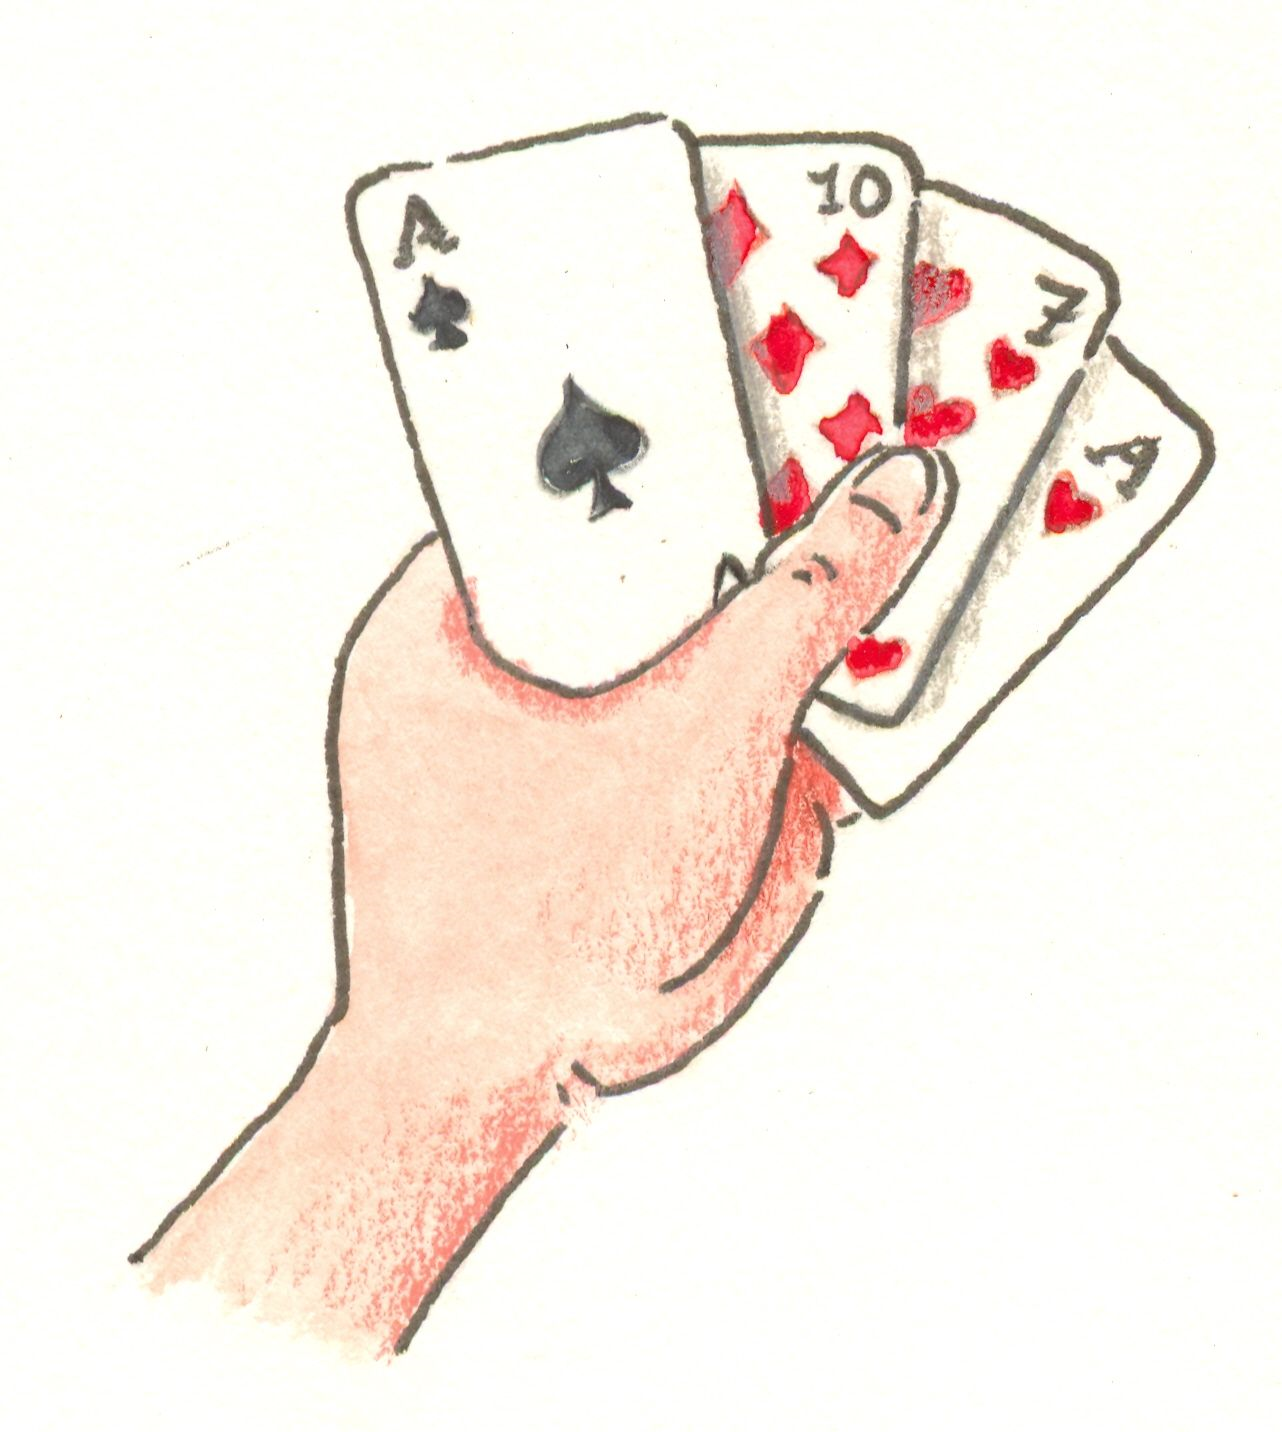
\includegraphics{kartenspiel}
\ \\
\ \\

\textbf{\textsc{\LARGE NET-WizHearts}}
\vspace{2cm}

\begin{tabular}{|c|c|c|}\hline
   Phase & Verantwortlicher & E-Mail \\ \hline\hline
   Pflichtenheft & Alina Meixl &  alina@meixl.de \\ \hline
   Entwurf & Viktoria Witka & witkaviktoria@freenet.de \\ \hline
   Spezifikation & Daniel Riedl & dariedl14@yahoo.de \\ \hline
   Implementation & Andreas Altenbuchner& a.andi007@gmail.com\\ \hline
   Verifikation & Patrick Kubin & kubin@fim.uni-passau.de\\ \hline
   Präsentation & w& w\\ \hline
 \end{tabular}

\end{center}

\end{titlepage}

\tableofcontents
\newpage

\section{Einleitung}
In diesem Dokument wird der konzeptionelle Entwurf des Online Multiplayer Kartenspiels NET-WizHearts dargestellt.\\
\ \\
Das Architektur-Diagramm verdeutlicht die Kommunikation zwischen Server und Client, die für die Anwendung von großer 
Bedeutung ist. Des Weiteren wird die Nutzung eines Regelwerkes veranschaulicht.\\
\ \\
Durch Angabe der Klassenstruktur wird eine erste Übersicht über die verschiedenen Komponenten des MVC-
Modells, welches der Anwendung zugrunde liegt, gegeben. Zu Illustrationszwecken werden außerdem einzelne Funktionsaufrufe
beispielhaft in Sequenzdiagrammen dargestellt.\\
\ \\
Durch das Verwenden des MVC Design Patterns wird eine Unabhängigkeit der View-Schicht 
vom restlichen System erzielt, so dass die graphische Oberfläche ohne Anpassung 
der Modell- und Controllerschicht auch für andere Regelwerke einsetzbar ist. Die Nutzung des Observer-Patterns erleichtert zudem
die Kommunikation zwischen der Modell- und View-Schicht.\\
\  \\



\section{Architektur-Diagramm}
Client-Server Diagramm. Der Client hat MVC Architektur.
\  \\
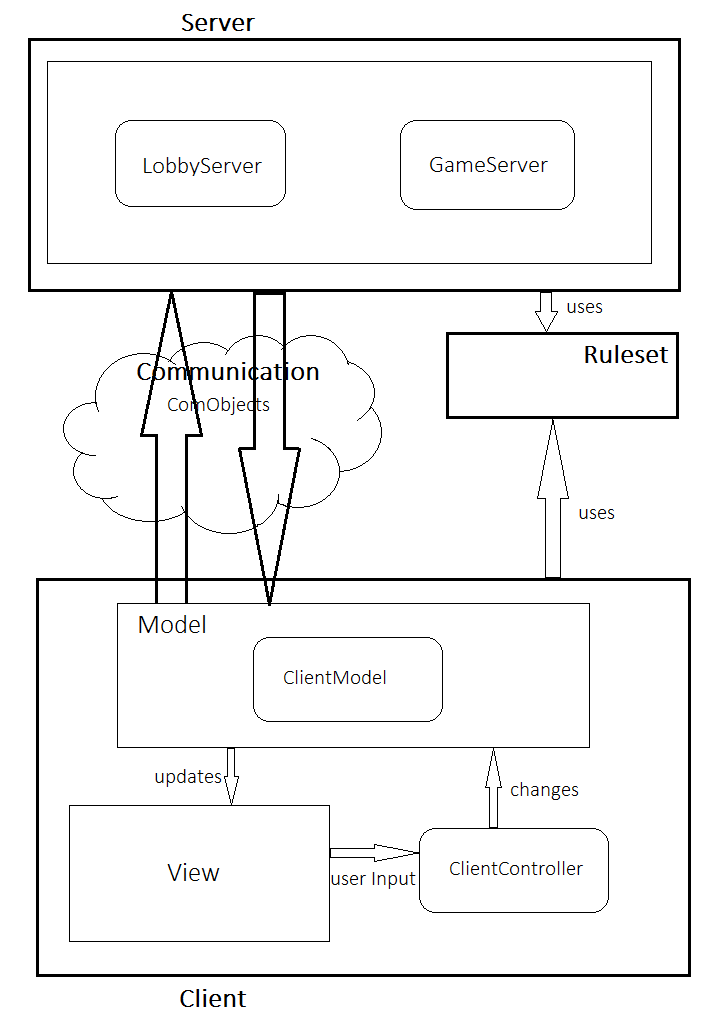
\includegraphics[height=15cm]{ArchitekturDiagramm}
\newpage
\section{Klassendiagramm}

\subsection{Packages}
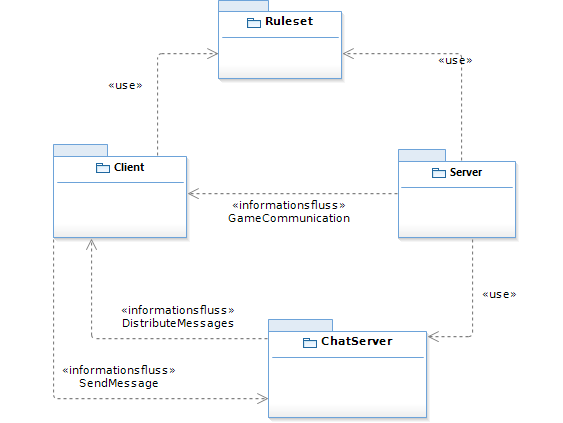
\includegraphics[width=\textwidth]{Packages}

\subsection{Server}
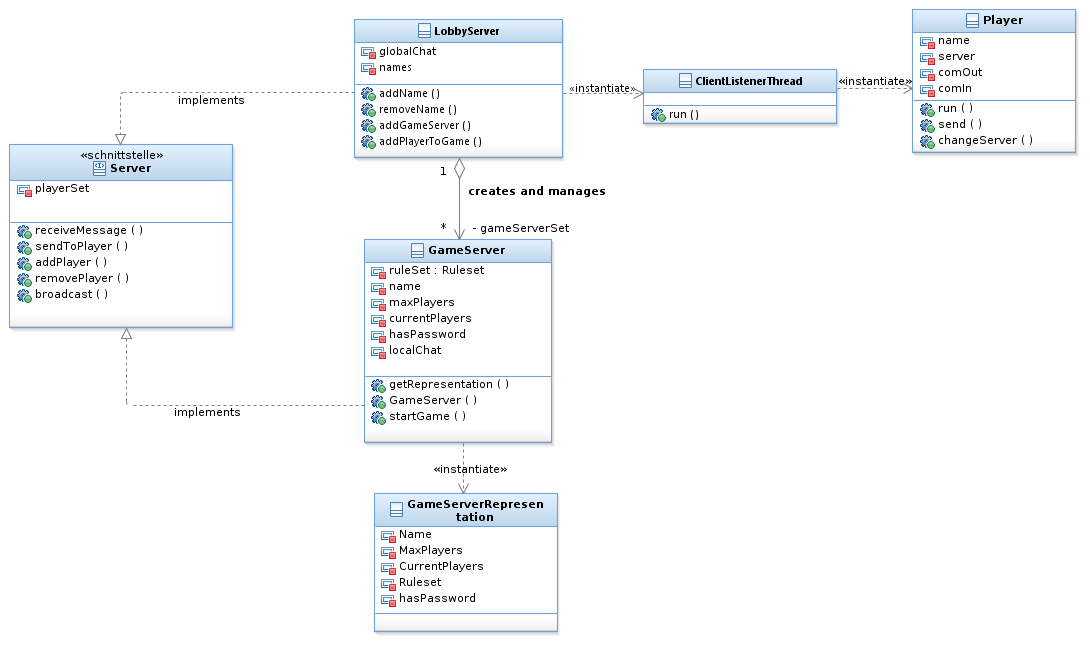
\includegraphics[width=\textwidth]{Server}
\textbf{ServerMain}: Diese Klasse startet den Server und ist für die Konfiguration und Wartung des Servers verantwortlich. \\

\textbf{Server} [interface]: Ist ein Interface das von den Klassen LobbyServer und GameServer implementiert wird. Es wird von den Klassen Player und Ruleset verwendet um Nachrichten und Befehle in Form von ComObjekten zu versenden. \\
		
\textbf{LobbyServer} [implementiert Server]: Diese Klasse ist für die Verwaltung der Spiellobby auf dem Server verantwortlich. Sie erstellt neue Spiele (/F126/) und verwaltet laufende Spiele (/L110/). Auch wird der Chatverkehr über sie an die verbundenen Spieler weitergeleitet. Die LobbyServer-Klasse implementiert das Server Interface um ComObjekte von Player erhalten zu können. Sie leitet Nachrichten in Form von ComObjekten an die verbundenen Spieler weiter. \\

\textbf{ClientListenerThread} [erbt von Thread]: Diese Klasse ist für das Zustandekommen von Clientverbindungen zuständig. Der ClientListenerThread wird von der Klasse LobbyServer instanziert und nach dessen Start wartet der Thread auf eingehende Clientverbindungen, stellt diese her und übergibt sie an Instanzen der Klasse Player, welche er ebenfalls instanziert. Der Player wird dann dem LobbyServer übergeben. \\

\textbf{GameServer} [implementiert Server]: Diese Klasse verwaltet ein Spiel ab dessen Erstellung bis zu seinem Ende. Sie leistet die Bereitstellung des Chatrooms im Spiel und verwaltet die Kommunikation zwischen den Clients während eines Spieles. Die GameServer-Klasse implementiert das Server Interface um Nachrichten von Player und Ruleset erhalten zu können. Der GameServer tauscht Nachrichten zwischen Ruleset und Player aus um so den Spielablauf zu koordinieren.\\

\textbf{Player} [erbt von Thread]: Die Player Klasse wird zum Versenden von Java Serializable Objects verwendet. Sie verwaltet für die Dauer einer Serververbindung den Socket zum Client. \\

\textbf{GameServerRepresentation} [implementiert Serializable]: Ist eine Klasse die Informationen über den Zustand eines Spielservers bereithält. Sie wird dem ComObjekt ComLobbyUpdateGameList angehängt um die Spielliste in der GameLobby zu aktualisieren.

\subsection{Client}
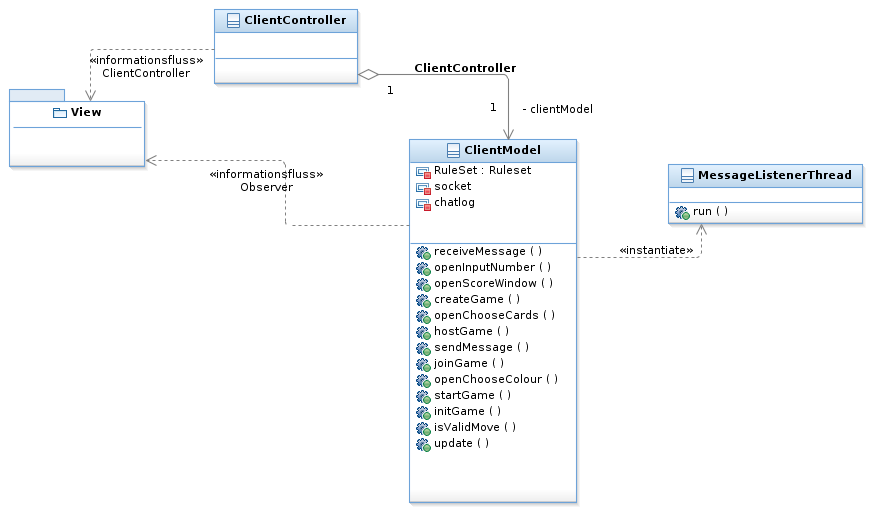
\includegraphics[width=\textwidth]{Client}
\textbf{ClientMain}: Dies ist die Hauptklasse des Clients, die beim Starten des Programmes ausgeführt wird. Sie erzeugt ein neues ClientController Objekt.\\

\textbf{Language} [Enumerator]: Language wird zur representation der Sprachen Deutsch, Englisch und Bayerisch im Client verwendet (/L350W/). \\

\textbf{ClientController}: Der ClientController enthält alle ActionListener der View und leitet durch diese Benutzereingaben an das ClientModel weiter.\\
Sobald der ClientController von der ClientMain Klasse erzeugt wird, erzeugt dieser wiederum das ClientModel und die ClientView, wobei zunächst nur das Login Fenster sichtbar ist. \\

\textbf{ClientModel} [erbt von Observable]: Das ClientModel ist die Schnittstelle zwischen dem MessageListenerThread, dem ClientRuleset und der View.\\ 
Das Model prüft Nachrichten, welche es vom MessageListenerThread über die Methode receiveMessage() bekommt. RulesetMessages werden an das Regelwerk weitergeleitet. Weiterhin informiert es die View über Veränderungen, indem sie MVMessages über notify() an die entsprechenden Observer schickt. Über sendMessage() können Kommandos vom Regelwerk oder der View, in Form von ComObjects, über den MessageListenerThreat an den Server gesendet werden.\\

\textbf{MessageListenerThread} [implementiert Runnable]: Der MessageListenerThreat wird vom ClientModel instanziert und hält die TCP-Verbindung zum Server. \\
Der Thread nimmt neue Nachrichten vom Server an und leitet sie an das ClientModel weiter, durch Aufruf von dessen receiveMessage() Methode.\\

\textbf{Window} [Enumerator]: Definiert die View-Klasse, für die die Nachricht bestimmt ist. \\

\textbf{MVMessage}: Diese Klasse stellt spezielle Objekte dar, welche bei der Kommunikation zwischen ClientModel und ClientView benötigt werden. Sie werden über notify() an die entsprechenden, über 'window' definierten, Observer geschickt, welche die passende Aktion ausführen. \\

\textbf{MVGameLobby} [erbt von MVMessage]: Nachricht, mit welcher die Spielerliste der GameLobby aktualisiert wird.

\textbf{MVLobby} [erbt von MVMessage]: Nachricht mit welcher die Spielerliste und Spielliste der Lobby aktualisiert wird.

\textbf{MVGame} [erbt von MVMessage]: Nachricht mit welcher das GamePanel des Game-Fensters aktualisiert wird.

\textbf{WizID} [Enumerator]: Repräsentationen der Wizard Karten auf View-Ebene

\textbf{HeartsID} [Enumerator]: Repräsentationen der Hearts Karten auf View-Ebene

\subsection{ClientView}
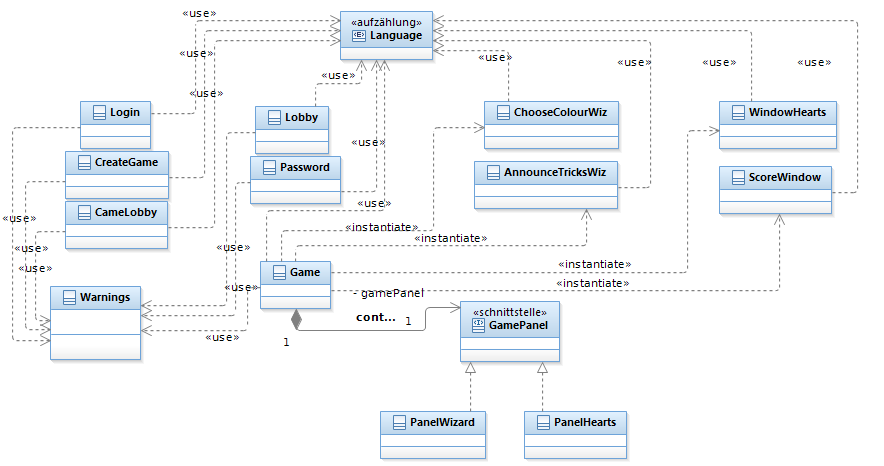
\includegraphics[width=\textwidth]{ClientView}
\textbf{MVMessages} [interface]:  Ist ein Interface, das von Lobby, GameLobby und Game implementiert wird. Es gibt eine Methode zur Verarbeitung von MVMessages vor. \\

\textbf{Login} [implementiert Observer]: Das Login-Fenster repräsentiert den initialen Dialog zwischen Benutzer und Client.
In diesem Fenster kann der Benutzer seinen Namen (/F042/) und die Adresse des Servers (/F040/) eingeben. Außerdem ist über den Login die Auswahl der Sprache möglich (/F050W/). Über den Login-Button wird die Verbindung zum Server hergestellt (/F045/).\\

\textbf{Lobby} [implementiert Observer, MVMessage]: Diese Klasse erzeugt die Ansicht der ServerLobby auf der Client Seite, in der die Spieler neue Spiele erstellen oder offenen beitreten können.\\
In der Lobby werden die Benutzernamen der sich in der Lobby befindenden Spieler(/L100/), sowie offene Spiele (/L110/) angezeigt. In der Lobby können Chatnachrichten gesendet (/F060/) und empfangen werden (/L115/). Über 'Leave' verlässt der Spieler das Spiel (/F090/). Über 'Host Game' (/F080/) wird der Spieler zum CreateGame Fenster weiter geleitet und mit 'Join Game' (/F070/) kann einem bereits erstellten Spiel beigetreten werden. \\

\textbf{CreateGame}: Das Fenster CreateGame dient dem Benutzer zur Erstellung eines neuen Spieles.\\
Es bietet alle Komponenten um ein Regelwerk zu wählen (/F120/), einen Spielnamen festzulegen (/F122/) und das Spiel durch ein Passwort zu schützen (/F130W/). In der Spielerstellung wird ein Titelbild des ausgewählten Spiels und eine kurze Beschreibung angezeigt (/L120/, /L122/). Über 'Leave' kehrt der Spieler in die Lobby zurück (/F124/) und mit 'Create' wird das Spiel erstellt (/F126/).\\

\textbf{Password [implementiert Observer]}: Dieses Fenster ermöglicht die Eingabe eines Passwortes (/F140W/) um einem Passwortgeschütztem Spiel beizutreten (/F142/) oder per 'Leave' wieder in die Lobby zurückzukehren (/F145/). \\

\textbf{GameLobby} [implementiert Observer, MVMessage]: Die GameLobby modelliert das Wartefenster, in dem beigetretene Spieler (/L155/) auf den Start des Spieles durch den Spielleiter warten (/F200/).\\
 Der Spielleiter kann Spieler mit dem Remove Player Button entfernen (/F180/). Über Leave kehren die Spieler in die Lobby zurück (/F170/, /F190/). Der spielinterne Chat ist ab hier verfügbar (/F160/, /L158/). \\

\textbf{Game} [implementiert Observer, MVMessages]: Im Game Fenster läuft das Spiel ab.\\
Es enthält den Spielchat (/F220/, /L260/) und ein GamePanel. Außerdem können über ein Dropdown-Menü Änderungen an Hintergrundbild und Kartenhintergründen vorgenommen werden(/F240).\\
Schließen beendet das Spiel und der Spieler wird in die Lobby zurückgeleitet (/F210/).\\

\textbf{GamePanel}: Das Panel ist die Komponente des Game-Fensters, welche das eigentliche Spiel darstellt.\\
Es besteht aus veschiedenen Panelobjekten, welche je nach Regelwerk auf das Spielfeld gezeichnet werden. \\
Dazu gehören die eigenen Karten (/L190/), eventuell ausgewählte Karten (/F225/, /F230/), ein Textfeld z.B. zur Anzeige der Anzahl der restlichen Karten der Mitspieler (/L192/) und den Ablagestapel (/L194/). Nach jeder Runde wird der Punktestand  aktualisiert (/L200/). \\

\textbf{OwnHand}: Stellt die Karten dar, die der Spieler auf der Hand hat. Der Spieler kann eine Karte durch Anklicken auswählen (/F225/) und durch einen zweiten Klick ausspielen (/F230/).\\

\textbf{OtherPlayer}: Zeigt die Informationen über die anderen Spieler, also den Namen, ein Symbol für die verdeckte Hand und das Label für zusätzliche Angaben an(/L198/). \\

\textbf{DiscardPile}: Stellt einen Ablagestapel dar, dieser kann sowohl für jeden Spieler einzeln oder für alle Spieler gemeinsam in der Mitte des Spielfeldes angezeigt werden.\\

\textbf{DrawDeck}: Stellt einen Aufnahmestapel dar. \\

\textbf{Warning} [implementiert Observer]: Das Warning-Fenster zeigt dem Benutzer Fehlermeldungen bzw. Hinweise an (/L290/), welche vom ClientModel übergeben wurden. Es wird nur im Fehlerfall angezeigt. \\

\textbf{ChooseItem}: Dieses Fenster ermöglicht es dem Spieler aus einer Liste von Items eines auszuwählen, wie beispielsweise die Trumpffarbe (/F360/). \\

\textbf{InputNumber}: In diesem Fenster, kann der Benutzer eine Zahl eingeben (/F370/). \\

\textbf{ChooseCards}: In diesem Fenster muss der Benutzer eine vorbestimmte Menge Karten auswählen (/F260/). \\

\textbf{ScoreWindow}: Dieses Fenster zeigt den momentanen Punktestand nach jeder Runde und den Gesamtpunktestand am Ende des Spieles an (/L250/).\\


\subsection{Ruleset}
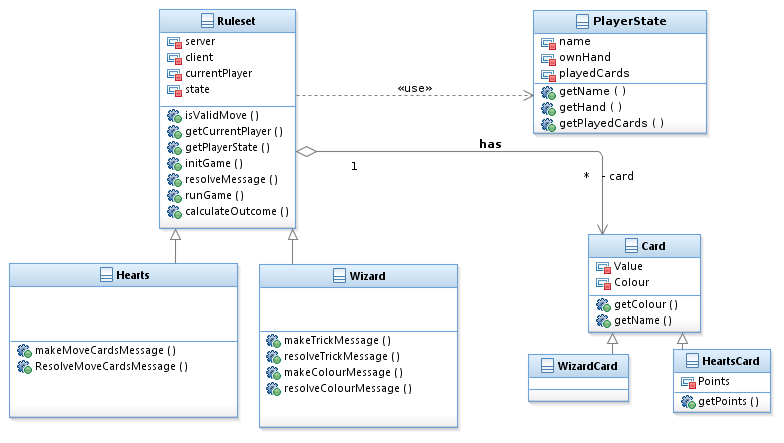
\includegraphics[width=\textwidth]{Ruleset}

\textbf{Ruleset} [Interface] Gibt die Methoden isValidMove() und resolveMessage() vor.

\textbf{ServerRuleset}[implementiert Runnable, Ruleset]: Das ServerRuleset  ist für den Ablauf und die Einhaltung der Regeln eines Spiels zuständig(/L280/). Das ServerRuleset wird im GameServer instanziert und verwaltet die Zustände des GameStates im Server. Mit der Methode isValidMove() wird eine Eingabe eines Clients auf Regelkonformität überprüft und dann im GameServer  das GameState verändert. Über resolveMessage() kann eine GameServerinstanz eine RulesetMessage vom Player an das Ruleset weiterleiten. \\ \\
		
\textbf{Hearts} [erbt von ServerRuleset]  Diese Klasse erstellt das Regelwerk zum Spiel Hearts. Sie enthält zudem weitere Methoden, welche für das Spiel Hearts spezifisch benötigt werden, wie die Regelung zum Tausch von Karten und die Berechnung der Stichpunkten. \\ \\
		
\textbf{Wizard} [erbt von ServerRuleset] Diese Klasse erstellt das Regelwerk zum Spiel Wizard. Sie enthält zudem weitere Methoden, welche für das Spiel Wizard spezifisch benötigt werden, wie das Bestimmen einer Trumpffarbe und die Bestimmung der Rundenanzahl. \\ \\
		
\textbf{ClientRuleset} [implementiert Ruleset]:  Das ClientRuleset wird zur Regelvorauswertung im Client verwendet. Dazu benutzt es die isValidMove() Methode. Desweiteren kann es vom ClientModel erhaltene RulesetMessages mit der resolveMessage() Methode behandeln.  \\

\textbf{ClientWizard} [erbt von ClientRuleset]: Diese Klasse bildet das Regelwerk für den Client bei einer Partie Wizard. \\

\textbf{ClientHearts} [erbt von ClientRuleset]: Diese Klasse bildet das Regelwerk für den Client bei einer Partie Hearts. \\
		
\textbf{GameState} Das GameState modelliert einen aktuellen Spielzustand, es wird vom GameServer instanziert und vom RuleSet bearbeitet. Es enthält die einzelnen PlayerStates, sowie Informationen zum Ablage-, Aufnahmestapel, Rundenanzahl, den momentanen aktiven Spieler sowie GamePhase. \\ \\
		
\textbf{GamePhase}[Enumerator] Die GamePhase modelliert die verschiedenen Zustände des Spiels im GameState. \\ \\
		
\textbf{PlayerState} [implementier Serializable] Repräsentiert den Spielzustand eines Spielers, und wird unter anderem im GameState gespeichert. Sie enthält den Namen des Spielers, seine Handkarten und OtherData. \\ \\
		
\textbf{GameClientUpdate} Das GameClientUpdate wird vom RuleSet über den GameServer an den Client geschickt und enthält alle Änderungen des GameState die für den Client relevant sind. Das wären sein Spielhand, der Ablagestapel sowie die Otherdata  von alle Spieler. \\ \\
		
\textbf{OtherData}[Abstrakt] [implementiert Serializable] OtherData speichert zu einem Spiel zusätzliche Informationen. \\ \\
		
\textbf{HeartsData} [erbt von OtherData] HeartsData speichert den Punktestand der Spieler. \\ \\
		
\textbf{WizData} [erbt von OtherData] WizData speichert die Trumpffarbe, sowie die vorausgesagten und gemachten Stiche der Spieler. \\ \\
		
\textbf{Card} [Abstrakt] [implementiert Serializable] Diese Klasse modelliert eine Spielkarte. Jede Karte besitzt als Attribute einen Wert und eine Farbe. \\ \\
		
\textbf{HeartsCard} [erbt von Card]  HeartsData modelliert eine Karte aus dem Spiel Hearts. \\ \\
		
\textbf{WizardCard} [erbt von Card] WizardData modelliert eine Karte aus dem Spiel Wizard. \\ \\

\subsection{ComObjects}
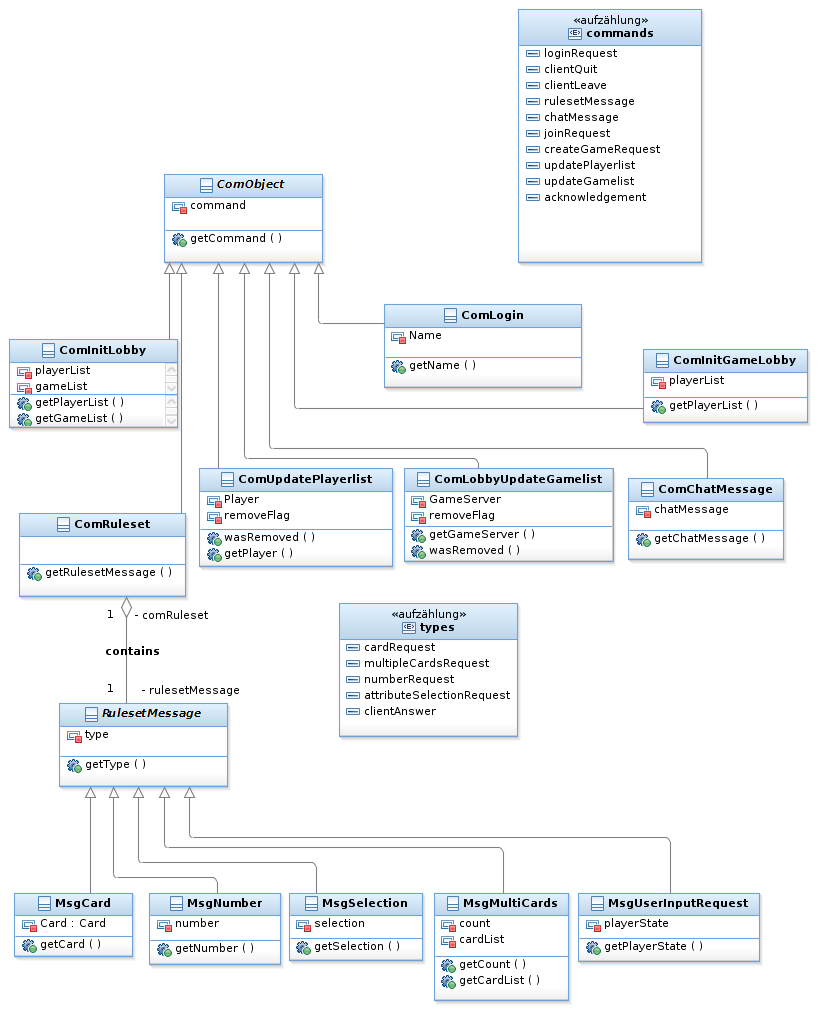
\includegraphics[width=\textwidth]{ComDiagram}
\textbf{ComObject} [implementiert Serializable]: Die Klasse ComObjekt ist eine Klasse, die ein Objekt darstellt, das zur Kommunikation genutzt werden kann. Sie enthält ein 'command', welches übermittelt, was passieren soll. Spezielle ComObjekt Klassen erben von dieser grundlegenden Klasse.\\

\textbf{ComInitLobby} [erbt von ComObjekt] Diese Klasse ist ein spezielles Kommunikations-Objekt. Sie synchronisiert den Client mit der Lobby, wenn er sich mit dem Server verbindet oder nach einem Spiel in die Lobby zurückkehrt. Dazu enthält sie sowohl die playerList, als auch die gameList.\\

\textbf{ComUpdatePlayerList} [erbt von ComObjekt] Diese Klasse ist ein spezielles Kommunikations-Objekt. Sie sendet eine Nachricht zum Update der Playerliste in der Lobby und Spiellobby. Dazu enthält sie den Player und ein removeFlag.\\
		
\textbf{ComLogin} [erbt von ComObjekt] Diese Klasse ist ein spezielles Kommunikations-Objekt. Sie ist eine Nachricht, die beim Login an den Server gesendet wird. Dazu enthält sie den Namen des Spieler, des sich einloggen möchte.\\
		
\textbf{ComLobbyUpdateGameList} [erbt von ComObjekt] Diese Klasse ist ein spezielles Kommunikations-Objekt. Sie aktualisiert die Gameliste in der Lobby. Dazu enthält sie den GameServer und ein RemoveFlag.\\
		
\textbf{ComInitGameLobby} [erbt von ComObjekt] Diese Klasse ist ein spezielles Kommunikations-Objekt. Sie liefert die Liste der Spieler, die sich bereits beim Betreten der Spiellobby darin befinden. \\

\textbf{ComJoinRequest} [erbt von ComObjekt] Diese Klasse ist ein spezielles Kommunikations-Objekt. Sie ist eine Nachricht, die an den Server gesendet wird, wenn der Spieler einem bestimmten Spiel beitreten will. Dazu enthält es den Namen des Spiels als String. \\
		
\textbf{ComChatMessage}[erbt von ComObjekt] Diese Klasse ist ein spezielles Kommunikations-Objekt. Sie enthält eine Chatnachricht in Form eines Strings.\\

\textbf{ComKickPlayer} [erbt von ComObjekt] Diese Klasse ist ein spezielles Kommunikations-Objekt. Sie ist eine Nachricht an den Server, die angibt einen Spieler vom Spiel zu entfernent. Dazu enthält es einene String der den Namen des Spielers enthält. \\
		
\textbf{ComRuleset} [erbt von ComObjekt] Diese Klasse ist ein spezielles Kommunikations-Objekt. Sie ist die grundlegende Nachricht eines Regelwerkaufrufes und enthält eine verfeinerte Nachricht mit weiteren Informationen, die RulesetMessage. \\
		
\textbf{RulesetMessage} [implementiert Serializable] Diese Klasse ist eine Verfeinerung der ComRuleset Klasse. Sie enthält einen Nachrichtentyp und vererbt an alle Nachrichten für das Regelwerk.\\
		
\textbf{MsgCard} [erbt von RulesetMessage] Diese Klasse ist eine Verfeinerung der ComRuleset Klasse. Sie beinhaltet die ausgespielte Karte eines Spielers.\\
		
\textbf{MsgNumber} [erbt von RulesetMessage] Diese Klasse ist eine Verfeinerung der ComRuleset Klasse. Sie enthält eine Zahl.\\
		
\textbf{MsgSelection} [erbt von RulesetMessage]Diese Klasse ist eine Verfeinerung der ComRuleset Klasse. Sie enthält die Wahl eines Items in Form eines Strings.\\
		
\textbf{MsgMultiCards} [erbt von RulesetMessage] Diese Klasse ist eine Verfeinerung der ComRuleset Klasse. Sie liefert mehrere Karten zum Tausch für das Regelwerk Hearts. \\
		
\textbf{MsgUser} [erbt von RulesetMessage] Diese Klasse ist eine Verfeinerung der ComRuleset Klasse. Sie wird dem Client gesendet, um eine Nutzereingabe anzufordern und/oder um dem ClientRuleset den aktuellen Spielzustand in Form eines GameClientUpdate zu übermitteln. \\

\textbf{MsgGameEnd} [erbt von RulesetMessage] Diese Klasse ist eine Verfeinerung der ComRuleset Klasse. Sie signalisiert dem ClientRuleset, dass das Spiel zu Ende ist.
		
\textbf{GameClientUpdate} [implementiert Serializable] Diese Klasse ist eine Verfeinerung der ComRuleset Klasse. Sie sendet den Aufruf, das Spiel zu updaten, nachdem eine Änderung passiert ist. \\
		
\textbf{enum commands} Enumerator, der ComObjekte ihre Kommandos zuweist. \\
		
\textbf{enum types} Enumerator zur eindeutigen Identifizierung von Regelwerknachrichten.
\ \\

\section{Sequenzdiagramme}
	\subsection{Spielstart}
		Mr. Blue, Mr. White und Mr. Pink befinden sich in der Lobby. \\
		Mr. Blue klickt auf 'New Game' und wird ins Erstellungsfenster geschickt. \\
		Er nimmt die nötigen Einstellungen vor (z.B. Wizard auswählen, Name setzen) und drückt auf 'Create'. Er wird ins Wartefenster weitergeleitet.\\
		Mr. Pink und Mr. White wählen Mr. Blues Spiel in der Lobby aus und drücken auf 'Join'. Sie werden an die Passwortabfrage geschickt.\\
		Sie geben das Passwort ein und werden ans Wartefenster geschickt.\\
		Die Mindestanzahl von drei ist erreicht. Mr. Blue drückt auf 'Start Game'.\\
		Mr. Blue, Mr. Pink und Mr. White werden ins Spiel geschickt. Das Spiel startet.\\

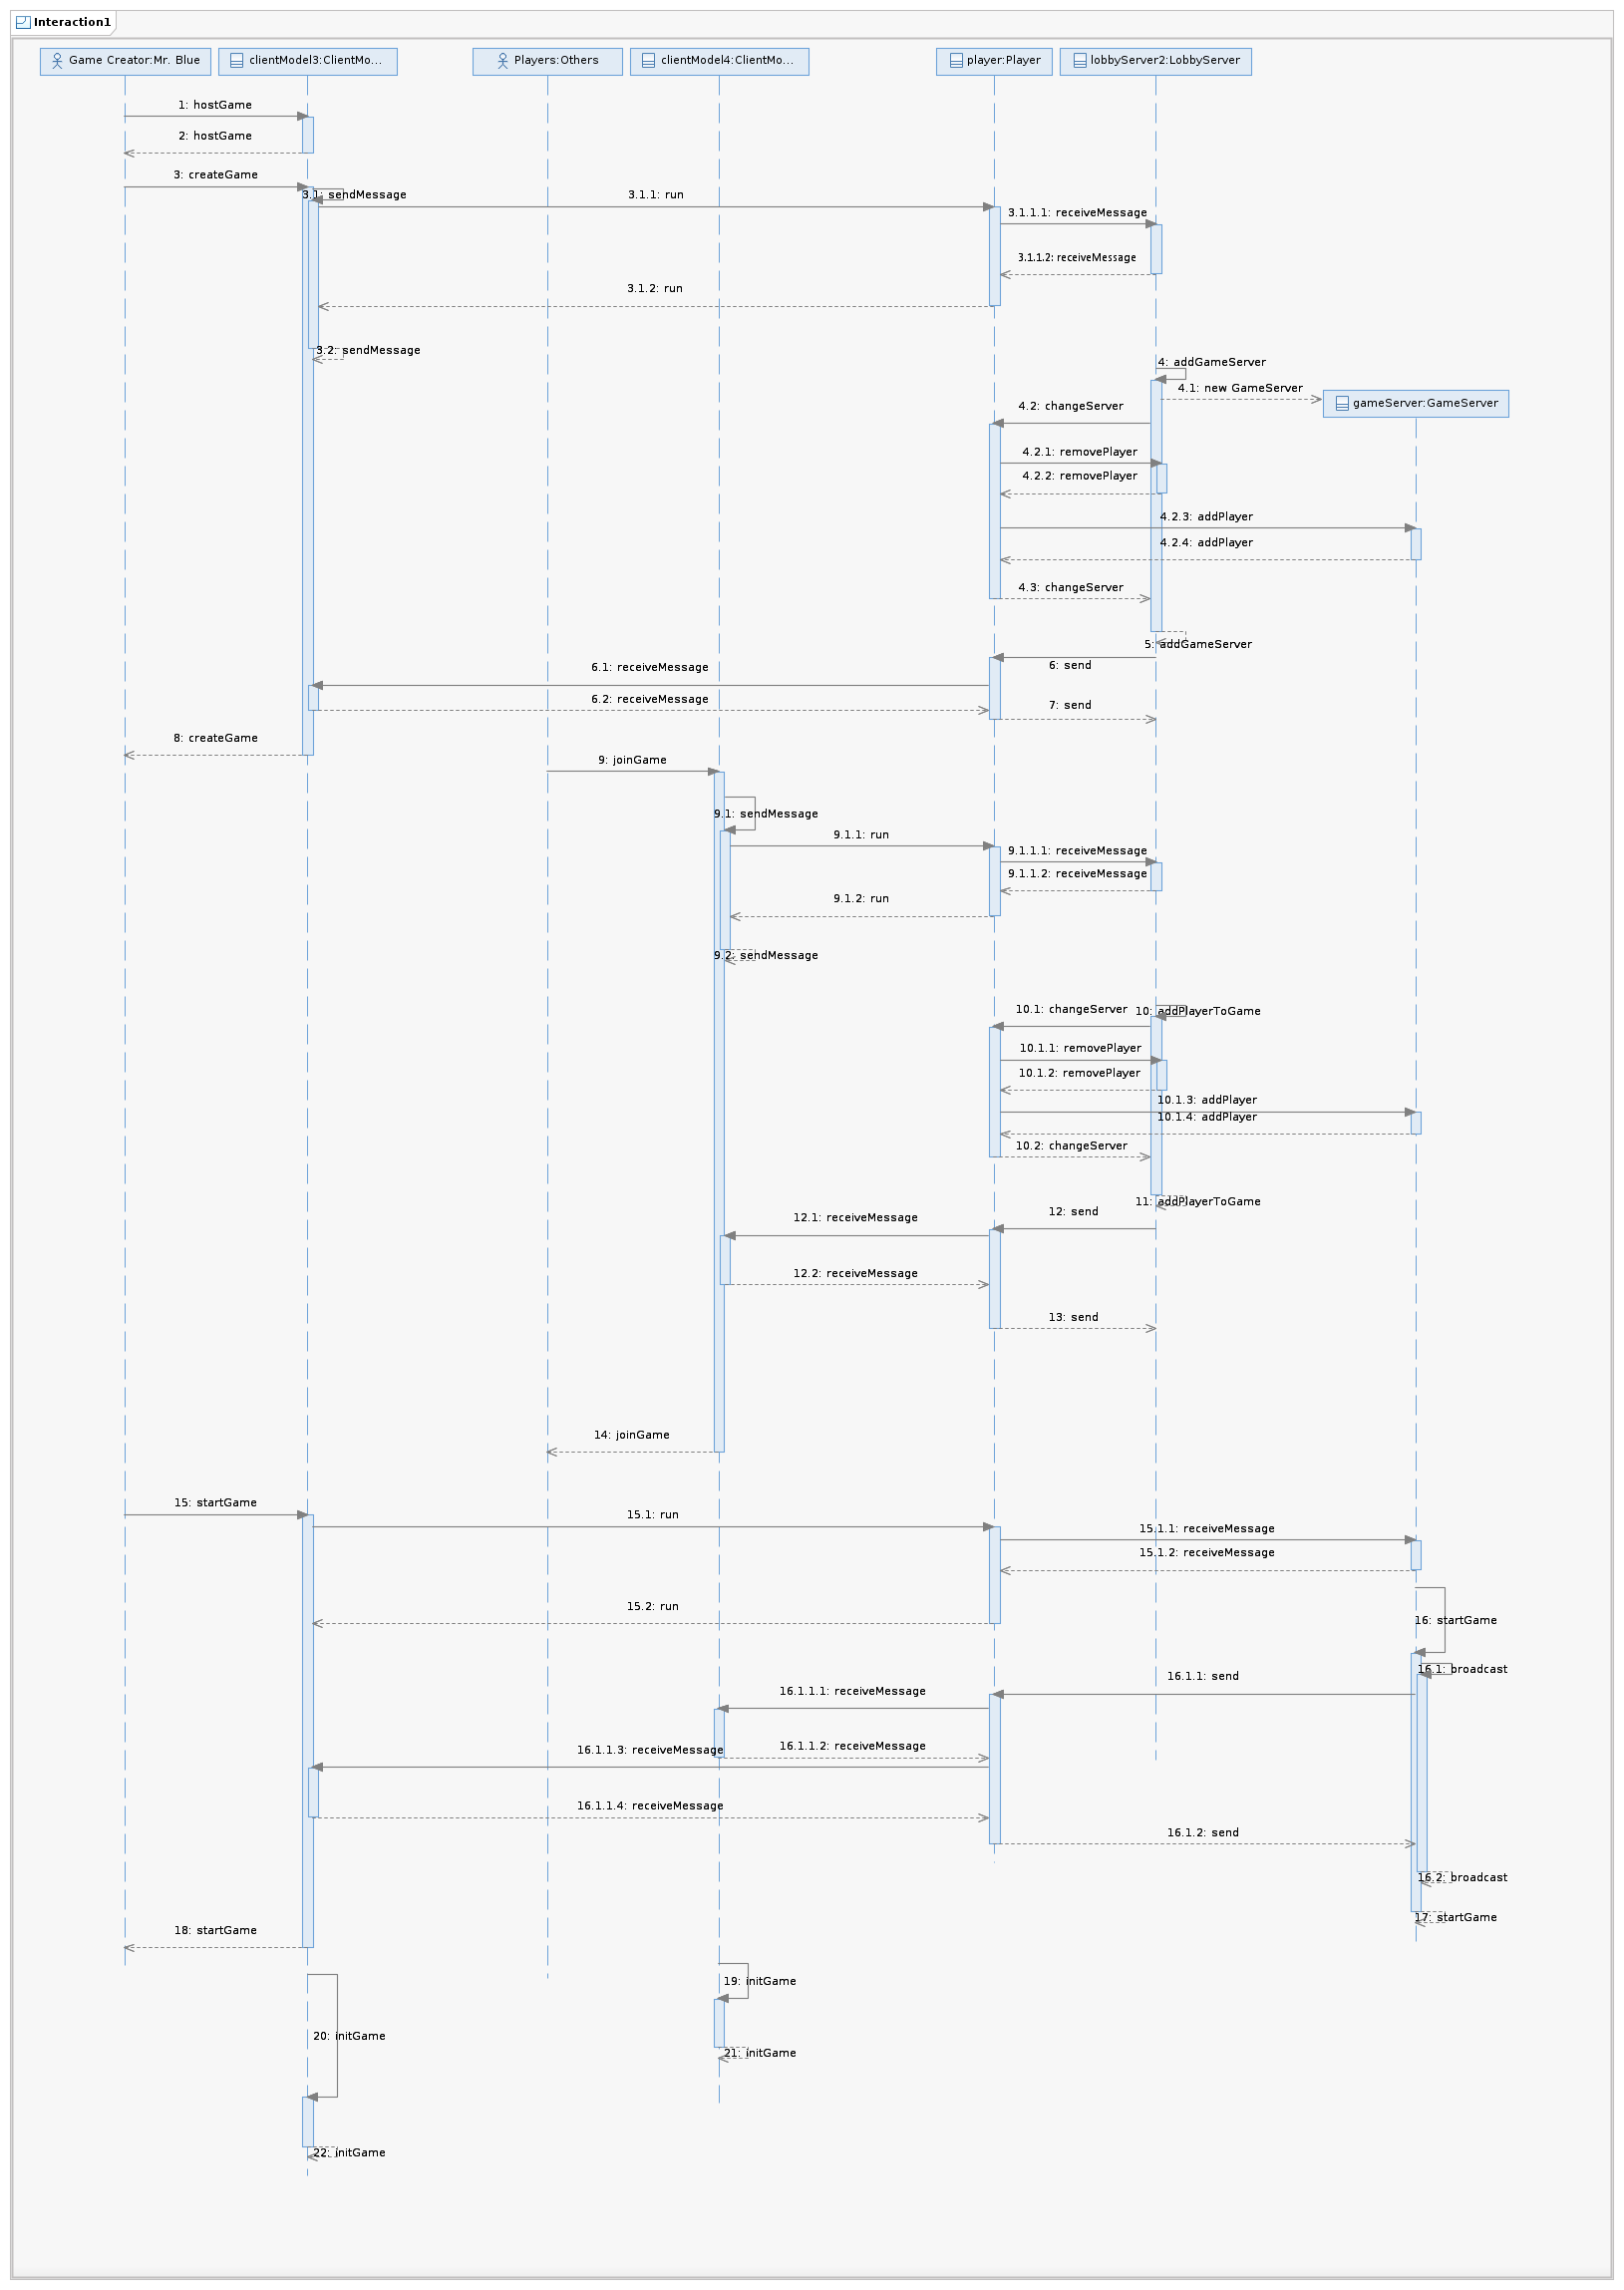
\includegraphics[width=\textwidth]{Entwurf_CreateGame}

\subsection{Spielzug}
		Aufgabe: Ein Spieler ist im Spiel Wizard an der Reihe und spielt eine Karte aus.
		Das Diagramm endet, sobald der Spielzug auf allen Clients sichtbar
		geworden ist und der nächste Spieler seinen Zug machen kann.\\
		\ \\
		Mr. Blue, Mr. White und Mr. Pink sind im Spiel Wizard. \\
		Mr. Blue ist an der Reihe, wählt eine Karte durch einmaliges Anklicken aus und spielt sie durch ein weiteres Anklicken.\\
		Der Zug wird auf Regelkonformität überprüft.\\
		Er ist nicht regelwidrig, also wird die gepielte Karte über den Server verschickt und bei Mr. Blue, Mr. Pink und Mr. White auf dem Ablagestapel angezeigt. \\
		Es wird überprüft, wer als nächstes dran ist.\\
		Der nächste Spieler ist am Zug. \\

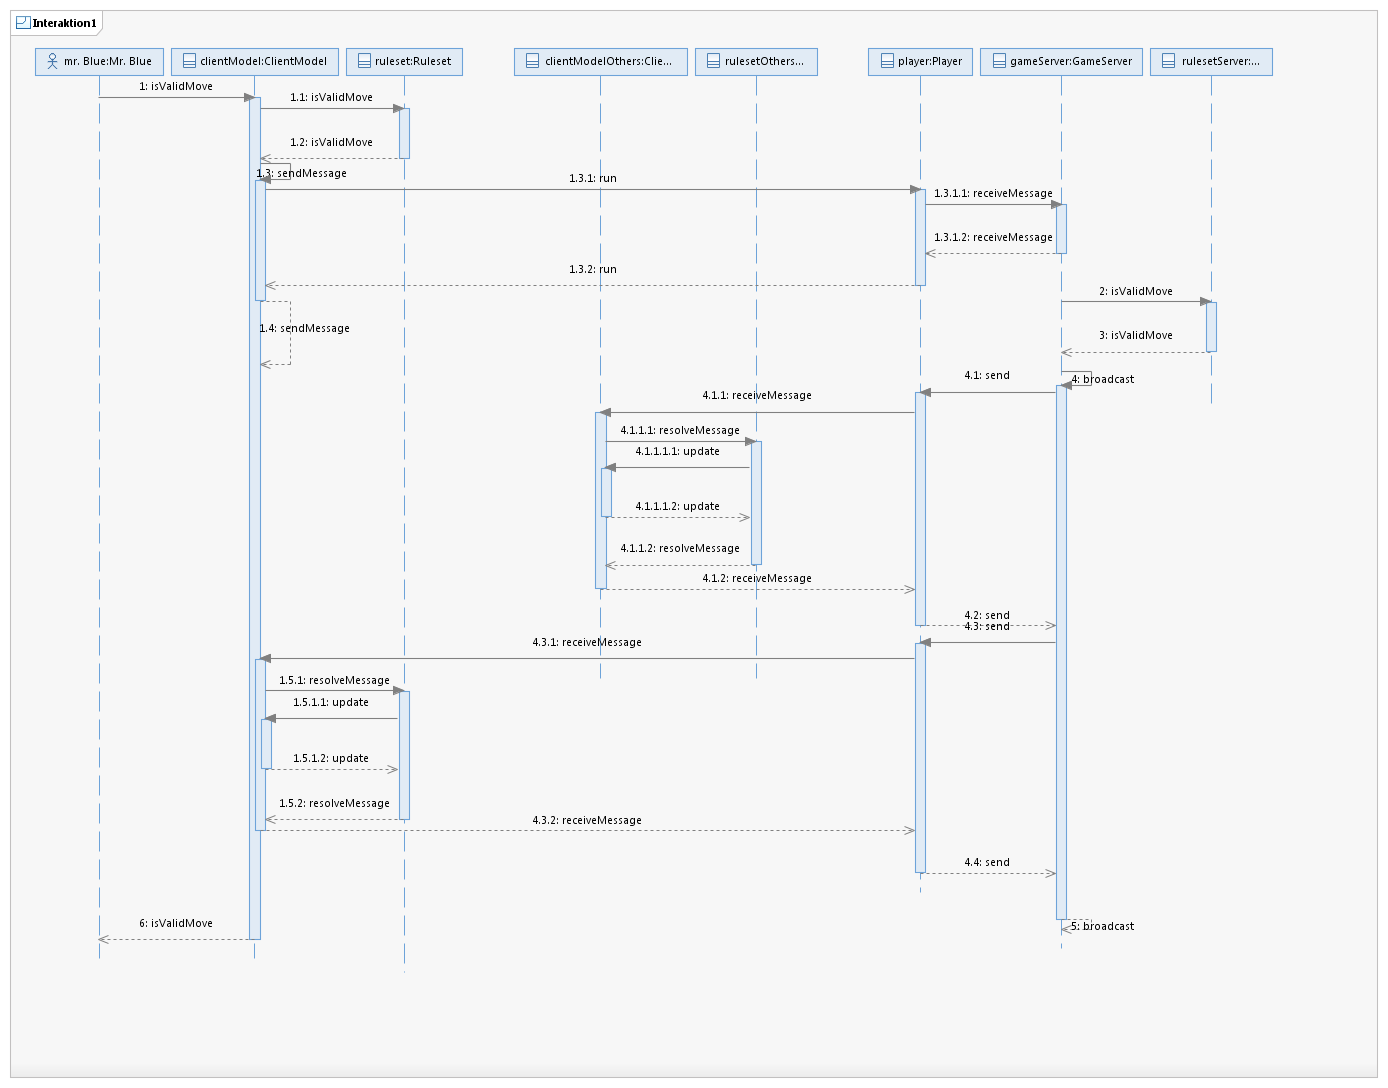
\includegraphics[width=\textwidth]{Entwurf_PlayCard}
		
\end{document}
